\documentclass[dvipsnames]{beamer}
\usepackage{tikz}
\usepackage{standalone}
\usepackage{wrapfig}
\usetikzlibrary{positioning, calc, shapes, fit, backgrounds, patterns}
\addtobeamertemplate{navigation symbols}{}{%
  \usebeamerfont{footline}%
  \usebeamercolor[fg]{footline}%
  \hspace{1em}%
  \insertframenumber/\inserttotalframenumber
}
\setbeamercolor{footline}{fg=NavyBlue}
\setbeamerfont{footline}{series=\bfseries}
\title{Hardware accelerator coupling in heterogeneous systems: an evaluation in the
  security domain}
\author{Bruno S M M Morais}
\date{December 10, 2019}

\begin{document}

\maketitle

\begin{frame}{Heterogeneous systems}
  \begin{itemize}
  \item Specialized HWACCs required for energy efficient embedded / edge computing
  \item Explosion in \# of ACCs in recent SoCs, specially with deployment of
    machine learning, DSP algorithms for instance
  \end{itemize}
\end{frame}

\begin{frame}{Loosely-coupled accelerators}
  \begin{columns}[T]
    \begin{column}{0.35\textwidth}
      \resizebox{0.35\textwidth}{!}{
        \begin{minipage}{0.5\textwidth}
          \centering
          \documentclass{standalone}
\usepackage[dvipsnames]{xcolor}
\usepackage{tikz}
\usetikzlibrary{positioning, calc, shapes, fit}

\begin{document}

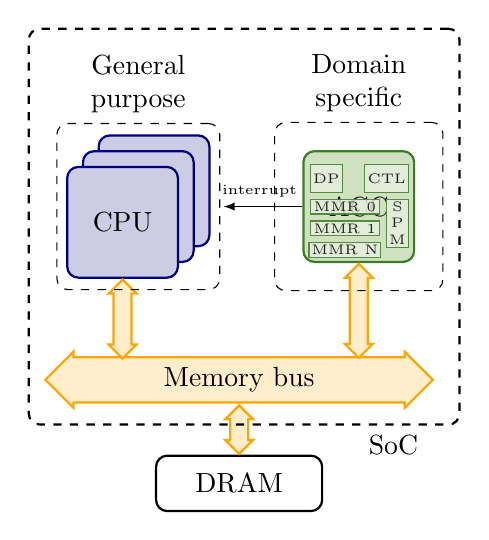
\begin{tikzpicture}
  \tikzstyle{PE}=[rounded corners, draw, thick, minimum size=40pt, align=center]
  \tikzstyle{core}=[PE, draw=NavyBlue, fill=NavyBlue!20]
  \tikzstyle{hwacc}=[PE, draw=OliveGreen, fill=OliveGreen!20]
  \tikzstyle{bus}=[double arrow, draw=Orange, fill=Orange!20, thick,
  minimum width=20pt, double arrow head extend=2pt]
  \tikzstyle{accint}=[draw=OliveGreen, fill=OliveGreen!10, outer sep=1pt, inner sep=1pt,
  node distance=0.5pt, opacity=0.85]

  \begin{scope}[name=soc, local bounding box=socbb]
  \node (core2) at (0.4,0.4) [core] {};
  \node (core1) at (0.2,0.2) [core] {};
  \node (core0) at (0,0) [core] {CPU};

  \node (hwacc1) at (3,0.2) [hwacc] {ACC};
  \begin{scope}[name=completeacc, local bounding box=accbb, shift={(3, 0.2)}]
    \node (reg0) [accint, minimum width=25pt, xshift=-5pt, minimum height=5pt, font=\tiny] {MMR 0};
    \node (reg1) [accint, minimum width=25pt, minimum height=5pt, below=of reg0, font=\tiny] {MMR 1};
    \node (reg2) [accint, minimum width=25pt, minimum height=5pt, below=of reg1, font=\tiny] {MMR N};
    \node (spm) [accint, minimum height=15pt, minimum width=5pt, align=center,
    right=of reg0.north east, font=\tiny, anchor=north west] {S\\P\\M};
    \node (accpe) [accint, minimum width=10pt, minimum height=10pt, above=of reg0.north west,
    anchor=south west, font=\tiny] {DP};
    \node (accctl) [accint, minimum width=10pt, minimum height=10pt, above=of spm.north east,
    anchor=south east, font=\tiny] {CTL};
  \end{scope}
  \node (mainbus) at (-1, -2) [bus, anchor=west, minimum height=140pt] {Memory bus};

  \node at (core0.south) [bus, rotate=90, anchor=east, scale=0.5, minimum height=57pt] {};
  \node at (hwacc1.south) [bus, rotate=90, anchor=east, scale=0.5, minimum height=68pt] {};

  \node (gpc) [fit=(core0)(core1)(core2), rounded corners,
  dashed, draw, minimum height=60pt, label={[align=center]90:{General\\ purpose}}] {};
  \node (dsc) [fit=(hwacc1), rounded corners, dashed, inner sep=10pt,
  draw, minimum height=60pt, label={[align=center]90:{Domain\\ specific}}] {};

  \draw[-latex] (hwacc1.west) -- ++(-1,0) node [anchor=south west, xshift=-4pt] {\tiny interrupt};
  \end{scope}

  \node (dram) [draw, rounded corners, below= of mainbus, minimum width=60pt,
  minimum height=20pt, yshift=10pt, thick] {DRAM};

  \node at (dram.north) [bus, rotate=-90, anchor=east, scale=0.5, minimum height=35pt] {};

  \node [fit=(socbb), draw, dashed, rounded corners, thick, inner sep=6pt, label={300:SoC}] {};

\end{tikzpicture}

\end{document}
        \end{minipage}
      }
    \end{column}
    \hfill
    \begin{column}{0.65\textwidth}
      \centering
      \begin{itemize}
      \item Access through shared memory bus
      \item Usually interrupts CPU when task is done
      \item With increase of \# of ACCs, communication becomes bottleneck
      \item CPU typically orchestrates compositions of HWACC functions
      \end{itemize}
    \end{column}
  \end{columns}
\end{frame}

\begin{frame}{Tightly-coupled accelerators}
  \begin{columns}[T]
    \begin{column}{0.5\textwidth}
      \begin{itemize}
        \item ACC moved into CPU datapath
        \item Requires ISA modification/extensions
        \item More difficult to explore, requires extensive modification of
          $\mu$Architecture and tools
      \end{itemize}
    \end{column}
    \hfill
    \begin{column}{0.5\textwidth}
      %\centering
      \resizebox{0.45\textwidth}{!}{
        \begin{minipage}{0.75\textwidth}
          \centering
          \documentclass{standalone}
\usepackage[dvipsnames]{xcolor}
\usepackage{tikz}
\usetikzlibrary{positioning, calc, shapes, fit, backgrounds}

\begin{document}
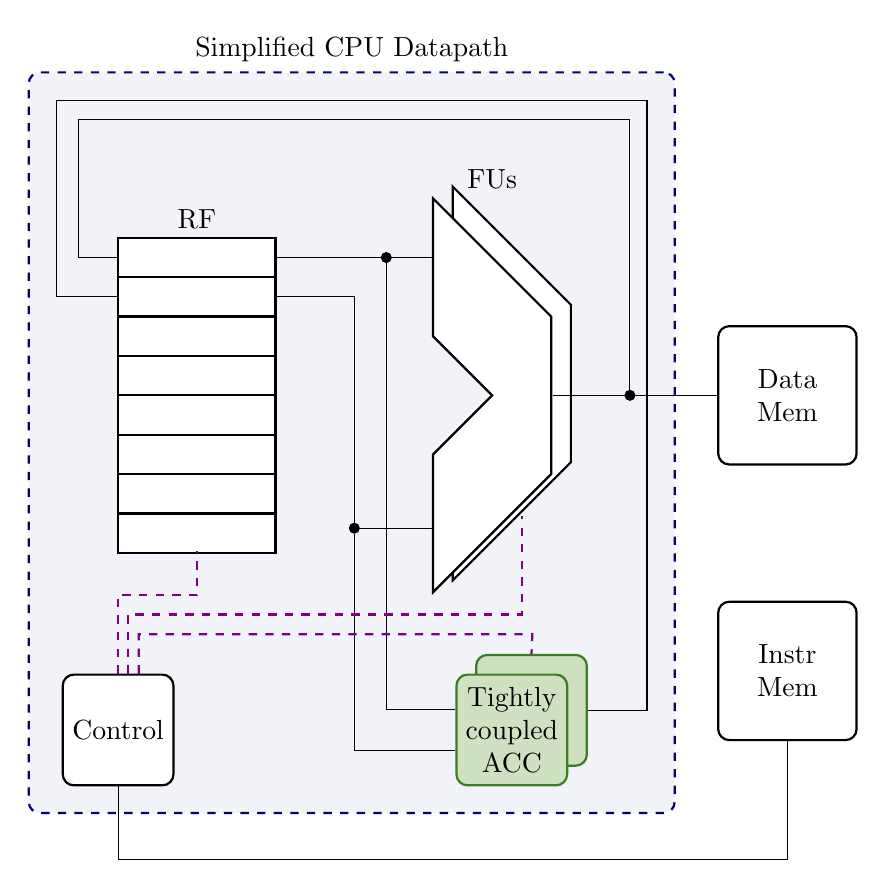
\begin{tikzpicture}
  \tikzstyle{coord}=[inner sep=0pt, outer sep=0pt, node distance=0pt]
  \tikzstyle{hwacc}=[rounded corners, draw=OliveGreen, fill=OliveGreen!20, thick, minimum size=40pt]
  \tikzstyle{control}=[draw=Purple, dashed, thick]
  \begin{scope}[name=datapath, local bounding box=dpathbb]

    % register file drawing
    \begin{scope}[name=rf, local bounding box=rfbb, shift={(0, -0.5)}]
      \node at (1,0) [anchor=south] {RF};
      \draw[fill=white, thick] (0,0) rectangle (2, -4);
      \foreach \i in {1,...,8} {
        \node (rfout\i) at (2, -0.5*\i+0.25) [coord] {};
        \node (rfin\i) at (0, -0.5*\i+0.25) [coord] {};
        \draw[thick] (0, -0.5*\i) -- (2, -0.5*\i);
      }
    \end{scope}

    % functional units
    \begin{scope}[name=fu, local bounding box=fubb, shift={(4, 0)}]
      \node at (0.75, 0) [anchor=south] {FUs};
      \begin{scope}[shift={(0.25, 0.15)}]
      \draw [fill=white, thick] (0, 0) -- (0, -1.75) -- (0.75, -2.5) -- (0, -3.25) -- (0, -5) -- (1.5, -3.5) -- (1.5, -1.5) -- cycle;
      \end{scope}
      \begin{scope}
        \draw [fill=white, thick] (0, 0) -- node [coord] (alua) {} (0, -1.75) -- (0.75, -2.5) -- (0, -3.25) -- node [coord] (alub) {}
        (0, -5) -- (1.5, -3.5) -- node [coord] (alux) {} (1.5, -1.5) -- cycle;
      \end{scope}
    \end{scope}

    % connections
    \draw (rfout1)  -| (alua);
    \draw (rfout2) -| ($(alub)!0.5!(rfout8)$) node (rfconn1) [coord, circle, fill=black, minimum size=4pt] {} -| (alub);
    \draw (alux) -- ++(1, 0) node (dataconn) [coord, circle, fill=black, minimum size=4pt] {} -- ++(0, 3.5) -- ++(-7, 0) |- (rfin1);

    % controller
    \node (ctl) at (0, -6.75) [draw, rectangle, rounded corners, minimum size=40pt, thick, fill=white] {Control};

    % tightly coupled acc
    \node (hwacc2) at (5.25, -6.5) [hwacc] {};
    \node (hwacc1) at (5, -6.75) [hwacc, align=center] {Tightly\\coupled\\ ACC};

    % accelerator connections
    \draw (hwacc2.east) -- ++(0.75, 0) -- ++(0, 7.75) -- ++(-7.5, 0) |- (rfin2);
    \draw (rfconn1) |- (hwacc1.200);
    \node (rfconn2) at (rfout1) [coord, circle, fill=black, minimum size=4pt, xshift=40] {};
    \draw (rfconn2) |- (hwacc1.160);
  \end{scope}

  \node (datamem) at (8.5, -2.5) [rounded corners, draw, thick, minimum size=50pt, align=center] {Data\\ Mem};
  \node (instmem) at (8.5, -6) [rounded corners, draw, thick, minimum size=50pt, align=center] {Instr\\ Mem};
  \draw (dataconn) -| (datamem.west);
  \draw (instmem.south) -- ++(0, -1.5) -| (ctl.south);

  % control lines
  \draw[control] (ctl.80) -- ++(0, 0.75) -- ++(5, 0) -- ++(0, 1.25);
  \draw[control] (ctl.90) -- ++(0, 1) -- ++(1, 0) -- ++(0, 0.55);
  \draw[control] (ctl.70) -- ++(0, 0.5) -- ++(1, 0);
  \draw[control] (ctl.70) -- ++(0, 0.5) -- ++(5, 0) -- (hwacc2.north);


  \begin{scope}[on background layer]
    \node [fit=(dpathbb), draw=NavyBlue, fill=NavyBlue!5, rounded corners, dashed, thick, inner sep=10pt,
    label={90:Simplified CPU Datapath}] {};
  \end{scope}
\end{tikzpicture}
\end{document}
        \end{minipage}
      }
    \end{column}
  \end{columns}
\end{frame}

\begin{frame}{RISC-V ecosystem}
  \begin{columns}[T]
    \begin{column}{0.6\textwidth}
      \begin{itemize}
      \item FOSS ISA specification and many implementations
      \item ISA is built to be extensible
      \item RoCC interface enables attaching HWACCs to datapath easily
        \begin{itemize}
        \item 4 custom opcodes for routing to 4 HWACCs
        \item Contents of two registers passed into HWACC
        \item Optionally response from HWACC written to a register
        \item Optional interface for requests into L1 cache
        \end{itemize}
      \end{itemize}
    \end{column}
    \hfill
    \begin{column}{0.4\textwidth}
      \centering
      
\includegraphics[width=0.75\textwidth]{media/Tall_2.pdf}
      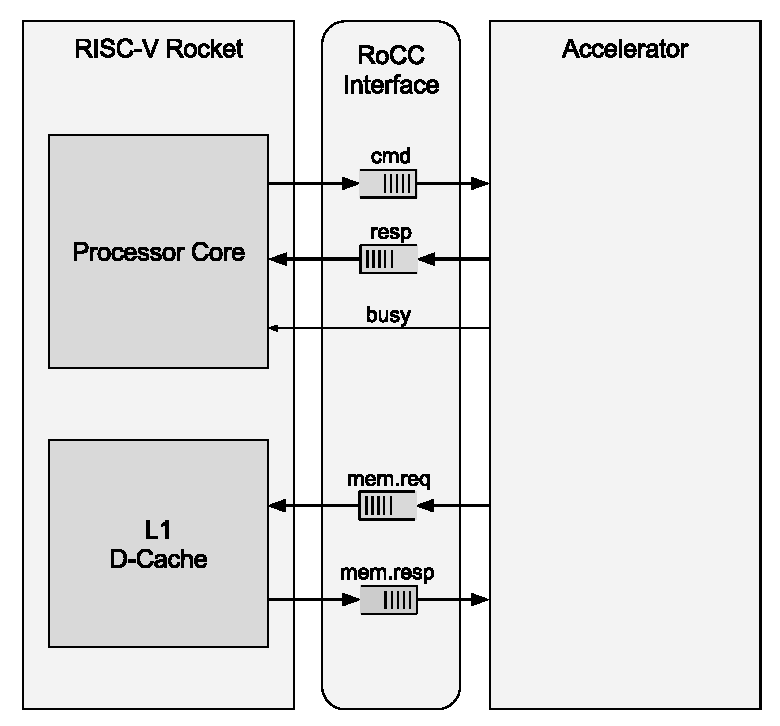
\includegraphics[width=1.0\textwidth]{media/rocc.pdf}
    \end{column}
  \end{columns}
\end{frame}

\begin{frame}{The Simon cipher family}
  \begin{columns}[T]
    \begin{column}{0.35\textwidth}
    \documentclass{standalone}
\usepackage[dvipsnames]{xcolor}
\usepackage{tikz}
\usetikzlibrary{positioning, calc, shapes, fit, backgrounds, patterns}

\begin{document}
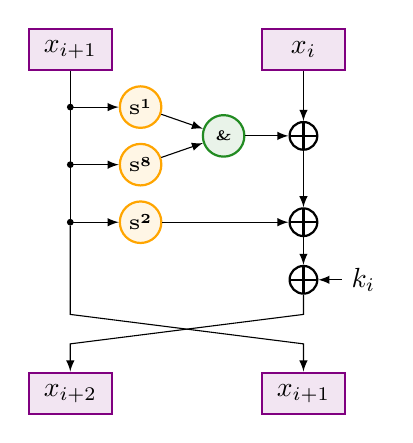
\begin{tikzpicture}
\tikzstyle{roundblock}=[draw=Purple, thick, fill=Purple!10, minimum width=30pt, minimum height=15pt]
\tikzstyle{function}=[draw=Orange, circle, thick, fill=Orange!10, minimum size=15pt,
font=\tiny\bfseries, node distance=5pt, inner sep=0pt]
\tikzstyle{XOR}=[draw,circle, minimum size=10pt, thick, append after command={
      [shorten >=\pgflinewidth, shorten <=\pgflinewidth,]
      (\tikzlastnode.north) edge[thick] (\tikzlastnode.south)
      (\tikzlastnode.east) edge[thick] (\tikzlastnode.west)},
    node distance=10pt]
\tikzstyle{junct}=[inner sep=0pt, circle, draw, fill=black, minimum size=2pt]

% inputs
\node (inpx) [roundblock] {$x_{i+1}$};
\node (inpy) [roundblock, right=of inpx, xshift=25pt] {$x_i$};

% shifts
\node (s1) [function, below=of inpx.south east, xshift=10pt] {S\textsuperscript{1}};
\node (s8) [function, below=of s1] {S\textsuperscript{8}};
\node (s2) [function, below=of s8] {S\textsuperscript{2}};

% and
\node (and) at ($(s1)!0.5!(s8)$) [function, draw=ForestGreen, fill=ForestGreen!10, xshift=30pt] {\&};

% xors
\node (xor1) at (and -| inpy) [XOR] {};
\node (xor2) at (s2 -| xor1) [XOR] {};
\node (xor3) [XOR, below=of xor2] {};

\node (key) [right=of xor3, xshift=-20pt] {$k_i$};

% connections
\draw[-latex] (s1) -- (and);
\draw[-latex] (s8) -- (and);
\draw[-latex] (and) -- (xor1);
\draw[-latex] (s2) -- (xor2);
\draw[-latex] (inpy) -- (xor1);
\draw[-latex] (xor1) -- (xor2);
\draw[-latex] (xor2) -- (xor3);
\draw[-latex] (inpx.south) |- node (junct1) [junct] {} (s1);
\draw[-latex] (junct1) |- node (junct2) [junct] {} (s8);
\draw[-latex] (junct2) |- node (junct3) [junct] {} (s2);
\draw[-latex] (key) -- (xor3);

% out
\node (outx) [roundblock,  below=of inpx, yshift=-80pt] {$x_{i+2}$};
\node (outy) [roundblock, right=of outx, xshift=25pt] {$x_{i+1}$};

\draw[-latex] (xor3.south) -- ++(0, -0.25) node (coord1) {} -- ([yshift=10pt]outx.north) -- (outx.north);
\draw[-latex] (junct3) -- (coord1 -| junct3) -- ([yshift=10pt]outy.north) -- (outy.north);


\end{tikzpicture}
\end{document}

    \end{column}
    \hfill
  \begin{column}{0.65\textwidth}
    \begin{itemize}
    \item Optimized for hardware implementations
    \item Only bitwise rotate, bitwise XOR and bitwise AND
    \item 64/128 (44 rounds) and 128/128 (128 rounds) configurations
    \end{itemize}
  \end{column}
  \end{columns}
\end{frame}

\begin{frame}{Hybrid crypto accelerator}
  \begin{columns}[T]
    \begin{column}{0.5\textwidth}
      \begin{itemize}
      \item Batch encrypt/decrypt
      \item Transparent encrypted memory load/store
      \item Direct access into coherent memory through DMA
      \item In this work, HWACC accesses into memory at L2 cache level
      \end{itemize}
    \end{column}
    \hfill
    \begin{column}{0.5\textwidth}
      % \centering
      \resizebox{0.3\textwidth}{!}{
        \begin{minipage}{0.5\textwidth}
          \centering
          
\documentclass{standalone}
\usepackage[dvipsnames]{xcolor}
\usepackage{tikz}
\usetikzlibrary{positioning, calc, shapes, fit, backgrounds, patterns}

\begin{document}
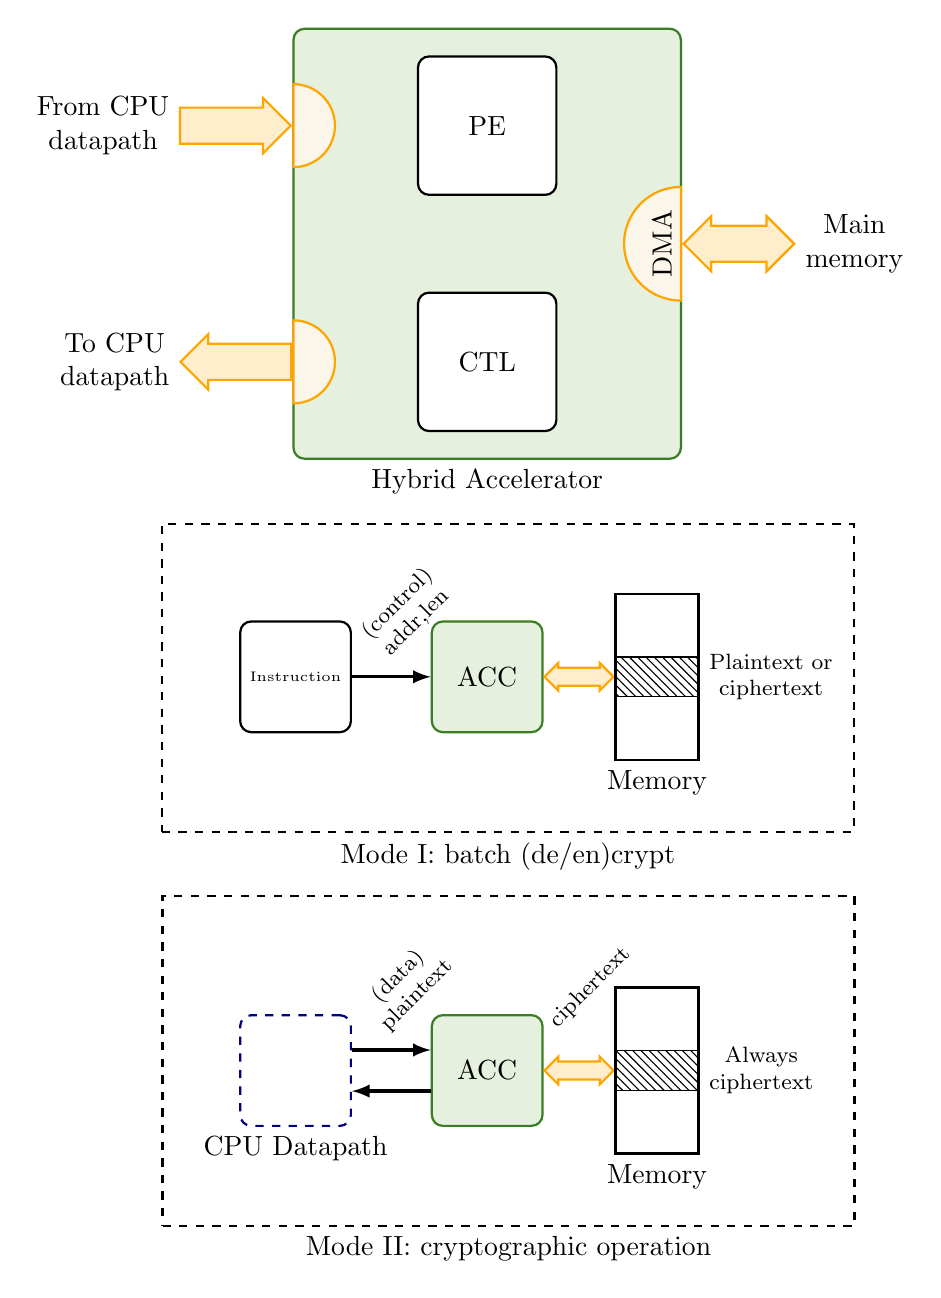
\begin{tikzpicture}
  \tikzstyle{accelement}=[rounded corners, draw, thick, minimum size=50pt, fill=white]
  \tikzstyle{port}=[semicircle, draw=Orange, fill=Goldenrod!10, anchor=south, thick]
  \tikzstyle{bibus}=[double arrow, draw=Orange, fill=Orange!20, thick,
  minimum width=20pt, double arrow head extend=2pt]
  \tikzstyle{ibus}=[single arrow, draw=Orange, fill=Orange!20, thick,
  minimum width=20pt, single arrow head extend=2pt]
  \tikzstyle{obus}=[single arrow, draw=Orange, fill=Orange!20, thick,
  minimum width=20pt, single arrow head extend=2pt, rotate=180]
  \tikzstyle{hwacc}=[rounded corners, draw=OliveGreen, fill=OliveGreen!10, thick]

  \begin{scope}[name=accstruct]
    \begin{scope}[name=acc, local bounding box=accbb]
      \node (accpe) [accelement] {PE};
      \node (accctl) at (0, -3) [accelement] {CTL};
    \end{scope}

    \begin{scope}[on background layer]
      \node (acc) [hwacc, fit=(accbb),
      minimum width=140pt, inner sep=10pt, label={270:Hybrid Accelerator}] {};
    \end{scope}

    \node (dmaport) at (acc.east) [port, minimum height=20pt, align=center,
    rotate=90] {DMA};
    \node (pathin) at (acc.west |- accpe.west) [port, rotate=270, anchor=south,
    minimum height=15pt] {};
    \node (pathout) at (acc.west |- accctl.west) [port, rotate=270, anchor=south,
    minimum height=15pt] {};

    \node (memconn) [bibus, anchor=west, minimum height=40pt, label={[align=center]0:{Main\\memory}}] at (dmaport.south) {};
    \node (fromdp) [ibus, anchor=east, minimum height=40pt, label={[align=center]180:{From CPU\\datapath}}] at (pathin.south) {};
    \node (todp) [obus, anchor=west, minimum height=40pt, label={[align=center]0:{To CPU\\datapath}}] at (pathout.south) {};
  \end{scope}

  \begin{scope}[name=op1, shift={(0, -7)}, local bounding box=mode1bb]
    \node (acc1) [hwacc, minimum size=40pt] {ACC};
    \node (inst) [draw, thick, rounded corners, left=of acc1, minimum size=40pt] {\tiny Instruction};
    \draw[-latex, very thick] (inst) -- node [anchor=south west, rotate=45, font=\footnotesize, align=center] {(control)\\addr,len} (acc1);
    \node (mconn1) at (acc1.east) [bibus, scale=0.5, anchor=west, minimum height=50pt] {};
    \node (dram1) at (mconn1.east) [draw, thick, minimum width=30pt, minimum height=60pt, anchor=west, label={270:Memory}] {};
    \draw [pattern=north west lines] (dram1.155) rectangle (dram1.335);
    \node at (dram1.east) [anchor=west, align=center, font=\footnotesize] {Plaintext or\\ciphertext};
  \end{scope}

  \node [draw,dashed, thick, fit=(mode1bb), inner sep=10pt, minimum width=250pt, label={270:Mode I: batch (de/en)crypt}, xshift=-12pt] {};

  \begin{scope}[name=op2, shift={(0, -12)}, local bounding box=mode2bb]
    \node (acc2) [hwacc, minimum size=40pt] {ACC};
    \node (dp) [draw=NavyBlue, thick, dashed, rounded corners, left=of acc2, minimum size=40pt, label={270:CPU Datapath}] {};
    \draw[-latex, very thick] (dp.20) -- node [anchor=south west, rotate=45, align=center, font=\footnotesize] {(data)\\plaintext} (dp.20 -| acc2.west);
    \draw[-latex, very thick] (dp.340 -| acc2.west) -- (dp.340);
    \node (mconn2) at (acc2.east) [bibus, scale=0.5, anchor=west, minimum height=50pt] {};
    \node (dram2) at (mconn2.east) [draw, thick, minimum width=30pt, minimum height=60pt, anchor=west, label={270:Memory}] {};
    \draw [pattern=north west lines] (dram2.155) rectangle (dram2.335);
    \node at (dram2.east) [anchor=west, align=center, font=\footnotesize] {Always\\ciphertext};
    \node at ([shift={(4pt, 30pt)}]mconn2) [align=center, rotate=45, font=\footnotesize] {ciphertext};
  \end{scope}

  \node [draw,dashed, thick, fit=(mode2bb), inner sep=10pt, minimum width=250pt,  label={270:Mode II: cryptographic operation}] {};

\end{tikzpicture}
\end{document}

        \end{minipage}
      }
    \end{column}
  \end{columns}
\end{frame}

\begin{frame}{Experimental setup}
  \begin{minipage}[0.2\textheight]{\textwidth}
    \begin{columns}[T]
      \begin{column}{0.8\textwidth}
        \begin{itemize}
        \item Three Simon accelerators
        \begin{itemize}
        \item MMIO (loosely-coupled)
        \item RoCC (tightly-coupled)
        \item RoCC + DMA (hybrid)
          \end{itemize}
        \end{itemize}
      \end{column}
      \begin{column}{0.2\textwidth}
        
\includegraphics[width=2.5cm]{media/cogs.jpeg}
      \end{column}
    \end{columns}
  \end{minipage}
  \begin{itemize}
  \item Both in-order (Rocket) and out-of-order (BOOM) cores
  \item SoC built with UC Berkeley's Chipyard (HWACCs attached)
  \item Performance: eight benchmarks run on SoC cycle-accurate simulations
    \begin{itemize}
    \item Software only: ECB and CBC mode
    \item MMIO accelerator, single: ECB and CBC mode
    \item MMIO accelerator, automatic: ECB mode
    \item Tightly-coupled accelerator: ECB and CBC mode
    \item Hybrid accelerator: ECB mode
    \end{itemize}
  \item Area \& power: HWACC synthesized for Xilinx FPGA, post-implementation
    metrics extracted
  \end{itemize}
\end{frame}

\begin{frame}{Results: performance}
  \begin{columns}[T]
  \begin{column}{0.5\textwidth}
  \includegraphics[width=1.0\textwidth]{media/ecb_speedup}
  \includegraphics[width=1.0\textwidth]{media/cbc_speedup}
  \end{column}
  \begin{column}{0.5\textwidth}
  \begin{itemize}
    \item Hybrid in batch mode is fastest, followed by regular MMIO
    \item Gains with RoCC accelerator, but is slower than 2-way BOOM SW only
    \item Need to understand RoCC interface timing better
    \item CBC mode performance very similar to EBC in comparable configurations
  \end{itemize}
  \end{column}
  \end{columns}
\end{frame}

\begin{frame}{Results: area \& power}
  \begin{itemize}
  \item Arty FPGA with 20800 LUTs / 41600 FFs available
  \item Usage reports 3119 LUTs and 2004 FFs, $\approx$ 17\% and 19.5\% of the
    total design (SoC) size
  \item Somewhat large usage due to unoptimized key expansion function
  \item ACC power consumption estimated at 8mW, $\approx$ 3\% of total SoC
    estimated power consumption (252mW)
  \item Key expansion function also accounts for most of power consumption at
    $\approx$ 87.5\% of ACC consumption
  \end{itemize}
\end{frame}

\begin{frame}{Future work}
  \begin{itemize}
  \item More flexible accelerators, multiple encryption modes, parallelized decryption
  \item Fully custom HWACC interface \& instructions, not RoCC
  \item Privileged HWACC access, OS support (multi-context)
  \end{itemize}
\end{frame}

\begin{frame}[allowframebreaks]{References}
  \tiny
  \nocite{*}
  \bibliography{paper}
  \bibliographystyle{ieeetr}
\end{frame}

\begin{frame}{Questions?}
  \centering
  \huge\bfseries ?
\end{frame}

\end{document}